\chapter{Allgemeine Grundlagen }
\label{chapter:allgemeine Grundlagen}


Das nachfolgende Kapitel behandelt die Grundlagen, die für ein Verständnis der Anwendungsbereiche von Apache Spark, dem Berkeley Data Analytics Stack und im Allgemeinen des Themenkomplexes Big Data Analytics und insbesondere für Machine-Learning-Anwendungen nötig sind. Im ersten Unterkapitel werden die grundsätzlichen Eigenschaften eines verteilten Systems beschrieben um die Basis für die in der Arbeit beschriebenen Besonderheiten von Verarbeitungen im Clusterbetrieb zu legen. Hier wird ein exemplarischer Clusteraufbau skizziert, Probleme mit Concurrency und Netzwerkverkehr beschrieben und welche Möglichkeiten es hier gibt.  Im darauf folgenden Unterkapitel werden grundlegende Problemstellungen und Technologien beschrieben, die im Rahmen von Big Data Analytics im Allgemeinen vorkommen. Unter anderem werden hier Grundlagen und Begriffe aus den Themengebieten Anwendungen von Big Data Analytics, Machine Learning, Klassifikation, Vorhersagen, statistische Analysen, Graph-Suchen und Streaming-Frameworks in erklärt. Besonders die Algorithmen, die in den Machine-Learning-Implementierungen MLibs und H20 zum Einsatz kommen, werden hier detaillierter vorgestellt. In einer Zusammenfassung werde diese Grundlagen nochmals auf einen Blick dargestellt. 
 

\section{Cluster Computing}
\label{section:cluster computing}

Die Nachfrage nach immer mehr Rechenleistung hat in dein letzten Jahren dazu geführt, dass verstärkt Rechnercluster eingesetzt werden. Alternativ gibt es den Ansatz, Mainframes\footnote{Unter Mainframe wird hier ein sehr leistungsfähiges Rechnersystem verstanden, das einen oder  beliebig viele Prozessoren in einer physischen Einheit, also einem logischen Mainboard verbindet. } mit immer mehr Rechenleistung auszustatten, diese jedoch ausdrücklich autonom zu betreiben\footnote{In diesem Kontext kann durchaus ein Failover-Cluster vorhanden sein, also eine Mainframe wird zur Ausfallsicherheit repliziert. Dies wird an dieser Stelle jedoch nicht als Cluster im eigentlichen Sinn bezeichnet.}. Je nach Aufgabenspektrum ist die eine oder andere Infrastruktur besser geeignet. In der Regel wird ein geclustertes System dort eingesetzt, wo hohe Verfügbarkeit oder gut parallelisierbare Aufgaben vorherrschen. Bei netzwerkintensiven Aufgaben, wie z.B. als Webserver oder Datenbanksystem sollten in der Regel besser Installationen auf einem autonomen System eingesetzt werden \citelit{clus1}.   

Ein Rechner-Cluster besteht in der Regel aus mehr oder weniger eng miteinander verbundenen Computern, wobei hier im Gegensatz zu Mainframes jeder Rechner über eigene Ressourcen wie Hauptspeicher, Massenspeicher, etc. verfügt. Ein Cluster, bzw. ein Verteiltes System ist nach Andrew S. Tanenbaum \citelit{tan1} folgendermaßen definert: 

\enquote{A distributed system is a collection of independent computers that appears to its users as a single coherent system.}

Bei der Verwendung eines Clusters sind einige Besonderheiten zu beachten, die bei der Ausführung auf gewöhnlichen Systemen nicht ins Gewicht fallen \citelit{tan1}. Unter Anderem sind die Tasks so gestalten, dass möglichst wenig Wartezeit durch Abhängigkeiten entsteht und diese möglichst autonom verarbeitet werden können. Außerdem muss beachtet werden, dass die einzelnen Knoten eines Clusters über Messaging-Mechanismen miteinander kommunizieren und dies insbesondere hohe Anforderungen an die Netzwerkinfrastruktur stellt. Eine typische Clustertopologie besteht aus mehreren Worker-Knoten und einem Masterknoten. Der Masterknoten deligiert die Tasks an die einzelnen Worker-Knoten und stellt das gesamte Cluster nach außen hin als ein geschlossenes System dar. Sämtliche Kommunikation mit dem Cluster findet grundsätzlich nur über den Masterknoten statt.


 
\section{Anwendungen für Big Data Analytics}
\label{section:anwendungen für big data analytics}

Im folgenden Unterkapitel werden exemplarisch einige Anwendungsfälle für \textit{Big Data Analytics} (auch \textit{Data Mining}) dargestellt, um zu klären, für welche Einsatzbereiche \textit{Frameworks} wie \textit{Apache Spark} und die darauf aufbauenden Bibliotheken in der Praxis benötigt werden.  

Laut Arvind Sathi \citelit{bda1} zeichnet sich \textit{Big Data} unter Anderem durch ein mögliches Vorkommen von unstrukturierten Daten aus. Die Autoren Chakraborty und Pagolu gehen in ihrem Artikel \citeint{ckb11} davon aus, dass mittlerweile mehr als 80\% der gesamten Daten im digitalen Raum in unstrukturierter Form vorliegen. In der Vergangenheit mussten für Analysetätigkeiten in aller Regel strukturierte Datensätze vorliegen. Grundsätzlich ist es mit den gängigen \textit{Data Analytics Frameworks} nach wie vor möglich, beispielsweise quantitative Analysen auf strukturierten Datensätzen durchzuführen oder unstrukturierte Datensätze nachträglich zu strukturieren, um wiederum quantitative Analysen darauf anwenden zu können.

Das Potential dieser \textit{Frameworks} zeigt sich jedoch dann in vollem Umfang, wenn auf unstrukturierten Daten diverse Analysemethoden oder Verarbeitungen angewendet werden. In jüngerer Vergangenheit ist das Aufkommen unstrukturierter Daten, wie bereits erwähnt, erheblich gestiegen. Dies wird nicht zuletzt durch die massive Verbreitung von Sensoren aller Art verursacht. Dies können \textit{Logdaten}, Bewegungsdaten, Sensorwerte zur Überwachung von technischen Einrichtungen, Messwerte aus Wetterstationen und unzähligen weiteren Quellen sein. Auch viele Internetanwendungen, besonders wenn es sich um laufende Datenströme handelt, verursachen erhebliche Datenmengen, die entweder \textit{persistiert} oder sogar zur Laufzeit analysiert werden können.  

\textit{Data Mining}\footnote{Ein Großteil der Literatur verwendet die Begriffe \textit{Big Data Analytics }und \textit{Data Mining} synonym. \textit{Machine Learning} wird jedoch von \textit{Data Mining} abgegrenzt, da letzteres eine explorative Datenanalyse darstellt.} ist laut \citelit{cl14} ein analytischer Prozess mit dem Zweck, große Datenmengen nach konsistenten Mustern oder systematischen Beziehungen zu untersuchen. Die Ergebnisse werden in der Regel validiert, in dem gefundene Muster oder Ähnlichkeiten auf einer Teilmenge der ermittelten Daten angewendet werden. Ein weiteres Ziel von \textit{Data-Mining-Prozessen} sind Vorhersagen von Ereignissen mittels geeigneter Algorithmen (Vergleich \citelit{cl14} und \ref{section:machine learning}). 

Der Prozess des Data Mining setzt sich nach \citelit{mit96} im Wesentlichen aus einem oder mehreren der folgenden Aufgabenbereiche zusammen:

\begin{itemize}
		\item \textbf{Klassenbeschreibung:} Eine knappe Beschreibung der Charakterisierung der Datensätze, um sie eindeutig von anderen Daten unterscheiden zu können. 
		\item \textbf{Assoziation:} Die Untersuchung der Daten nach assoziativen Verbindungen oder Korrelationen zwischen einzelnen Daten oder Datengruppen.   
		\item \textbf{Klassifizierung:} Hier wird ein definierter Satz von Trainingsdaten\footnote{Trainingsdaten können beispielsweise Daten sein, die bereits im Vorfeld manuell klassifiziert wurden, deren Klassenzugehörigkeit also bekannt ist.} analysiert und anhand deren Beschaffenheit ein Modell generiert. Durch die Klassifizierung werden Entscheidungsbäume (siehe Kapitel \ref{section:machine learning}) oder Klassifizierungsregeln generiert, die schließlich für die Klassifizierung folgender Daten verwendet werden \citelit{pdl97}. 
		\item \textbf{Vorhersage:} Die Vorhersage bezieht sich auf mögliche Werte von nicht-vorhandenen Daten oder Datenspektren, die wiederum durch \textit{Approximation} einer Funktion mittels Beispielen durchgeführt wird \citelit{cl14}. Dies sind ebenfalls Trainingsdaten, die aus Datensätzen mit den dazugehörigen berechneten Funktionswerten bestehen. 
		\item \textbf{Cluster-Analyse:} Diese dient dazu, \textit{Cluster} innerhalb von Datensätzen zu ermitteln. Dies sind Daten, die definierte Ähnlichkeiten zueinander aufweisen. 
		\item \textbf{Zeitreihenanalysen:} Hier werden in der Regel große Mengen an Zeitreihendaten analysiert, um nach Ähnlichkeiten oder Mustern innerhalb der Daten zu suchen.  
		
\end{itemize}	

\newpage


\section{Machine Learning}
\label{section:machine learning}

\enquote{Learning denotes changes in the system that are adaptive in the sense that they enable the system to do the same task (or tasks drawn from a population of similar tasks) more effectively the next time.} \citelit{sim83}

Unter \textit{Machine Learning} wird ein interdisziplinärer Teilbereich der Informatik und der Statistik verstanden. Ziel ist die Erstellung von Algorithmen, die in der Lage sind, selbstständig auf Grund von Daten iterativ zu lernen gemäß der oben zitierten Definition. Um dies zu erreichen, erstellen diese Algorithmen basierend auf den jeweiligen Eingabedaten Modelle, die Entscheidungen oder Vorhersagen treffen können \citelit{isl13}. In den Abbildungen \ref{fig:MLP1} und \ref{fig:MLP2} wird dies veranschaulicht. 


\begin{figure}[htb!]
\centering
\begin{tikzpicture}[node distance=2cm]
\tikzstyle{line} = [draw, -latex']

\node (start) [startstop] {Training Data};
\node (pro2b) [block, right of=start, xshift=2cm] {\textbf{Pre-Processing} \\-Normalization \\ -Dimension Reduction};
\node (pro3b) [block, right of=pro2b, xshift=2cm] {\textbf{Learning} \\-Supervised \\ -Unsupervised};
\node (pro4b) [block, right of=pro3b, xshift=2cm] {\textbf{Error Analysis}\\ -Precision/Recall \\ -Overfitting};
\node (pro5b) [process, below of=start] {Model};

\path [line] (start) |- (pro2b);
\path [line] (pro2b) |- (pro3b);
\path [line] (pro3b) |- (pro4b);
\path [line] (pro4b) |- (pro5b);


\end{tikzpicture}
\caption{Der Machine-Learning-Prozess: Phase 1 - Lernphase}
\label{fig:MLP1}
\end{figure}


\begin{figure}[htb!]
\centering

\begin{tikzpicture}[node distance=2cm]
\tikzstyle{line} = [draw, -latex']

\node (pro5b) [process] {Model};
\node (pro6b) [startstop, below of=pro5b] {Data};
\node (pro7b) [block, right of=pro5b, xshift=2cm, yshift=-1cm] {\textbf{Prediction}};
\node (pro8b) [startstop, right of=pro7b, xshift=2cm] {Predicted Data};

\path [line] (pro5b) |- (pro7b);
\path [line] (pro6b) |- (pro7b);
\path [line] (pro7b) |- (pro8b);

\end{tikzpicture}
\caption{Der Machine-Learning-Prozess: Phase 2 - Prediction-Phase (Vorhersage)}
\label{fig:MLP2}
\end{figure}

Das erste Diagramm \ref{fig:MLP1} zeigt den Lernprozess. Zunächst werden definierte Trainingsdaten einem \textit{Pre-Processing}\footnote{Das Pre-Processing kann aus \textit{Normalisierung, Dimensionsreduktion, Bildverarbeitung} oder anderen Vorarbeiten bestehen.} zugeführt (Vergleich Unterkapitel \ref{section:klassifikationsalgorithmen}). 

Danach folgt der eigentliche Lernprozess, der mit oder ohne \textit{Überwachung}\footnote{Beim überwachten Lernen (Supervised Learning) liegen der Analyse vorher angelegte Trainingsdaten zugrunde, das unüberwachte Lernen (Unsupervised Learning) erzeugt vorher gänzlich unbekannte Modelle aus gefundenen Mustern \citeint{ul04}}, als \textit{Minimalisierungsfunktion} oder mit anderen Lernalgorithmen durchgeführt wird (siehe Unterpunkte Clusterverfahren und Klassifikationsalgorithmen). Der Lernprozess kann entweder mit einem bestimmten Lernalogrithmus durchgeführt werden, oder mit sogenannten \textit{Ensemble-Learning-Methods}. Dies ist die Zusammenfassung von unterschiedlichen Lernalgorithmen zu einem Lernprozess, um die Vorhersageleistung zu steigern. Nach dem Lernprozess werden das erzeugte Modell einem Validierungsprozess zugeführt. Dies können \textit{Precision/Recall}\footnote{\textit{Precision:} Wie viele der ausgewählten Datensätze sind relevant. \textit{Recall:} Wieviele relevante Datensätze wurden ausgewählt. }, \textit{Overfitting}\footnote{\textit{Overfitting} bezeichnet einen Zustand, in dem bekannte Daten (Trainingsdaten) von einem Algorithmus generell akkurater erkannt werden, als Daten, die von dem Algorithmus erkannt werden sollen (Predicitions).}, oder andere Validierungsfunktionen sein. Am Ende der Prozesse entsteht ein Modell, das für verschiedenste Aufgaben eingesetzt werden kann. 

In Abbildung \ref{fig:MLP2} wird das erzeugte Modell zusammen mit produktiven Daten genutzt, um mittels geeigneter Vorhersagealgorithmen (siehe Unterkapitel \ref{section:vorhersagealgorithmen}) bisher noch nicht vorhandene Datensätze erzeugen zu können.  

Die Hauptanwendungsgebiete für \textit{Machine Learning} sind sämtliche Bereiche, in denen eine Anwendung von strikten, regelbasierten Algorithmen nicht in Frage kommt \citelit{pdl97}. Beispiele für diese Bereiche sind laut \citelit{pml06} Suchmaschinen, Sprach- und Musikerkennung, Handschriftenerkennung, Spamfilter, Umgebungserkennungen und viele mehr. 



\subsection{Klassifizierung von Daten}
\label{section:klassifizierung von daten}


Im Gegensatz zu herkömmlichen \textit{Business-Intelligence-Anwendungen}\footnote{Laut \citelit{bi12} versteht man unter \textit{Business Intelligence (BI)} die Sammlung, Auswertung und Darstellung von Daten anhand definierter Prozesse.} zeichnen sich Big-Data-Anwendungen in erster Linie durch Unterschiede in der Herangehensweise und in der Formulierung der primären Fragestellungen aus. In der Vergangenheit wurden zu Beginn einer Analyse zunächst Problemstellungen formuliert und aufgrund dessen Prozesse und vor allen Dingen die zu sammelnden Daten definiert \citelit{bi12}. Mit der steigenden Etablierung von Big-Data-Anwendungen hat sich dieser Ansatz gewandelt. Hier werden zunächst sämtliche anfallenden Daten gespeichert. Auf diese Datensätze, deren Größe in relativ kurzer Zeit massiv anwachsen kann, werden erweiterte Analyseprozesse\footnote{Unter dem Begriff \textit{Advanced Analytics} sind verschiedene Werkzeugtypen aus der vorhersagenden Analyse (\textit{Predictive Analytics}), aus dem Data Mining, aus der Statistik, der Künstlichen Intelligenz, der Sprachverarbeitung und weiteren Disziplinen zusammengefasst \citelit{tdwi11}.} angewendet, die unter anderem auch Vorhersagen erlauben \citelit{tdwi11}. 
So liegen also bei Big-Data-Analytics große Datenmengen vor, ohne dass das Ziel der Analyse im Vorfeld bekannt ist. 

\subsubsection{Clusterverfahren}
\label{section:clusterverfahren}

Nun gibt es verschiedene Herangehensweisen, wie sich relevante Fragestellungen aus den vorliegenden Daten ableiten lassen. Ein sinnvoller Ansatz besteht darin, sogenannte Cluster innerhalb der Daten zu ermitteln, also ähnliche Datensätze zu entsprechenden Gruppen zusammenzufassen. Aus diesen Gruppen werden Klassen gebildet, in dem ihnen aussagekräftige Namen zugeordnet werden\citelit{cl14}. Cluster werden beispielsweise benötigt, um Kunden nach bestimmten Interessen zu gruppieren, um Zeichen auf Ähnlichkeiten für die automatischen Zeichenerkennung zu untersuchen, oder Bilder auf vergleichbare Bildpunktanordnungen oder Farbspektren, also generell überall, wo nach Ähnlichkeiten gesucht wird. 

Ein Cluster zeichnet sich dadurch aus, dass die Objekte innerhalb eines Clusters möglichst ähnlich sind, die Cluster untereinander jedoch möglichst unähnliche Inhalte besitzen. Um Ähnlichkeiten zwischen Datensätzen oder Clustern feststellen zu können, bedarf es einer Distanzfunktion, zur Ermittlung und Sicherstellung der Clustergüte einer Qualitätsfunktion (Vergleich \citelit{cl14}). 

Laut \citelit{cl14} sind für Distanz- und Qualitätsfunktionen folgende Annahmen zu treffen:  


\begin{framed}
\begin{flalign*}
&\textbf{Vorbedingungen}& \\
&X \text { (Instanzenraum) }&  \\
&E \subseteq X \text{ (Instanzenmenge) }& \\
&X\times X \to \mathbb{R}^+ \text{ (Abstandsfunktion) }&  \\
&2^{2^x} \to \mathbb{R} \text{ (Qualitätsfunktion) }& 
\end{flalign*}

Gesucht wird eine Clustermenge \(C = \{C_1,...,C_k\}\) \text{mit folgenden Eigenschaften:} \\

\(C_i \subseteq E\) \\
\(quality(C) \to max\) \\
\(C_i \cap C_j = \emptyset\) \\
\(C_1 \cup...\cup C_k = E\) \\



Die Abstandsfunktion \(dist\), die gegebene Objekte so in Teilmengen zerlegt, dass der Abstand der Objekte innerhalb einer Teilmenge (Cluster) kleiner ist, als der Abstand zu Objekten anderer Teilmengen: \\

\(\forall C_i, C_j \in C(i \neq j) : \forall x_k, x_l \in C_i, x_m \in C_j : dist(x_k, x_l) < dist(x_k, x_m)\)\\

Die Qualitätsfunktion \(quality\) beschreibt die Qualität des Clusterings basierend auf der Abstandsfunktion \(dist\): \\

\({quality}(C = \{C_1 \subseteq E,...,C_k \subseteq E\}) \to \mathbb{R}\) \\ 
\end{framed}

\newpage

Exemplarisch werden im Folgenden einige Distanzfunktionen dargestellt, die für die Clusteranalyse wichtig sind (Vergleich \citelit{uma14},  \citelit{bro98}):

\begin{itemize}
\item \textbf{Hamming-Distanz:} Hier werden die Vektorelemente der Position \(i\) zweier Vektoren miteinander verglichen. Wenn sich diese unterscheiden, wird die Distanz auf den Wert 1 gesetzt, bei gleichen Werten 0. Nachdem alle Elemente der Vektoren miteinander verglichen wurden, werden diese summiert. Ein Vorteil der Hamming-Distanz ist, dass sich Abstände zwischen metrischen, ordinalen und sogar nominalen Daten berechnen lassen. Der Nachteil dieser Distanzfunktion ist, dass Abstandsverhältnisse nicht erkannt werden, also ist beispielsweise der Abstand zwischen 2 und 3 für diese Funktion gleichwertig zum Abstand von 2000 zu 2100.

\(dist_H(x,y) = count_i(x_i \neq y_i) \)

\item \textbf{Manhattan-Distanz:} Diese Distanzfunktion hat ihren Namen aufgrund der blockweisen Anordnung der Straßenzüge in Manhattan. Distanzen werden, wie auf einem Schachbrett, durch vertikale und horizontale Bewegungen und Richtungsänderungen beschrieben. Um die Ergebnisse der verschiedenen Distanzfunktionen untereinander vergleichbar zu machen, wird der Betrag der Distanzwerte verwendet. Die Manhattan-Distanz ist nur auf metrische Daten anwendbar. Diese Distanzfunktion ist auch unter dem Namen \textit{Block-Distanz} bekannt.   

\(dist_M(x,y) = \sum_{i} \mid x_i - y_i \mid \)


\item \textbf{Euklidische Distanz:} Hier wird der direkte Abstand zwischen zwei Vektoren beschrieben, also zweier Punkte im n-dimensionalen Raum. Diese Funktion lässt sich nur auf metrische Daten anwenden. Auch hier wird durch Quadrieren und der Quadratwurze der Differenzen eine Normalisierung erreicht, die die Distanzwerte vergleichbar macht. 

\(dist_E(x,y) = \sqrt{\sum_{i}(x_i - y_i)^2} \)

\item \textbf{Tschebyscheff-Distanz:}  Auch hier wird der Abstand zwischen zwei Punkten im n-dimensionalen Raum betrachtet. Im Unterschied zu den beiden vorhergehenden Verfahren wird hier jedoch der größtmögliche absolute Abstand zwischen allen Attributen ermittelt. Deshalb wird diese Distanzfunktion auch als \textit{Maximum-Distanz}  bezeichnet. 

\(dist_T(x,y) = max_i(\mid x_i - y_i \mid) \)

\item \textbf{Minkowski-Distanz:}  Diese Distanz-Funktion ist ähnlich zur Euklidischen Distanz. Allerdings entspricht hier der Abstand der \(n\)-ten Wurzel der Summe der  \(n\)-ten Potenzen der Differenzen. Auch diese Funktion lässt sich nur auf metrische Daten anwenden.

\(dist_K(x,y) = \sqrt[n]{\sum_{i}(x_i - y_i)^n} \)

\end{itemize}

Darüber hinaus existieren noch zahlreiche weitere Distanzfunktionen, die je nach Einsatzzweck besser oder schlechter geeignet sein können, als die dargestellten. 


\newpage


Die Clusteranalyse zählt zu den \textit{unüberwachten Lernalgorithmen (Unsupervised Learning)}. Zoubin Ghahramani beschreibt dies in seinem Artikel \textit{Unsupervised Learning} \citeint{ul04} wie folgt: 

\enquote{[...]in unsupervised learning the machine simply receives inputs x1, x2,..., but obtains neither supervised target outputs, nor rewards from its environment. It may seem somewhat mysterious to imagine what the machine could possibly learn given that it doesn’t get any feedback from its environment. However, it is possible to develop of formal framework for unsupervised learning based on the notion that the machine’s goal is to build representations of the input that can be used for decision making, predicting future inputs, efficiently communicating the inputs to another machine, etc. In a sense, unsupervised learning can be thought of as finding patterns in the data above and beyond what would be considered pure unstructured noise.}

Prinzipiell wird zwischen vier verschiedenen Clusterarten unterschieden \citelit{cl14}: 

\begin{itemize}
		\item \textbf{Partitionierendes Clustering:} Eine Menge von Datenobjekten wird in k Cluster, die um einen Medoid\footnote{Medoide sind Stellvertreterobjekte eines Clusters, deren durchschnittliche Ähnlichkeit zu allen Datenobjekten des Clusters maximal ist. Ein Medoid ist immer ein Datensatz aus dem Cluster.} oder einen Centroid\footnote{Centroide sind Vektoren der Mittelwerte der Attribute aus den Datenobjekten. Im zweidimensionalen Raum entspricht dies der Mittelwerte der x- und y-Koordinaten aller Datenobjekte.} gebildet werden, zerlegt (Vergleich \citeint{km11}). 
		\item \textbf{Hierarchisches Clustering:} Hier werden die Cluster hierarchisch aufgebaut, indem jeweils die Cluster mit der größten Ähnlichkeit, also mit der geringsten Distanz, miteinander vereinigt werden. Aus diesen vereinigten Clustern können in der Hierarchie übergeordnete Ebenen entstehen. Beim \textit{Agglomerativen Clustering} wird mit den einzelnen Datenobjekten selbst begonnen, in dem jedes Cluster aus genau einem Datenobjekt besteht. Die jeweils ähnlichsten Cluster werden vereinigt und somit zu einer neuen Hierarchieebene. Dies geschieht so lange, bis in der obersten Ebene ein Cluster mit allen Datenobjekten entstanden ist. Beim \textit{Divisiven Clustering} wird die Hierarchie in umgekehrter Reihenfolge aufgebaut, also zunächst werden alle Datenobjekte zu einem großen Cluster zusammengenommen und dieser dann iterativ anhand der  Ähnlichkeiten der Datenobjekte untereinander geteilt.  
		\item \textbf{Dichtebasiertes Clustering:} Die Cluster werden so gebildet, dass in der Umgebung eines Datenobjektes innerhalb eines Clusters möglichst viele weitere Datenobjekte liegen, die Dichte also besonders hoch ist. Die geforderte Dichte wird über Schwellenwerte definiert. 
		\item \textbf{Clustering mit Neuronalen Netzen:} Auch über neuronale Netze können Cluster gebildet werden. Die Netze werden in diesem Fall nicht überwacht trainiert (Vergleich Einleitung Kapitel \ref{section:machine learning}) und nutzen das Verfahren des \textit{Wettbewerbslernens} (Vergleich \citelit{cl14}, beispielsweise \textit{Vonoroi-Mengen}). Das Neuron, welches dem Eingabewert (dem Datenobjekt) am ähnlichsten ist, ist im jeweiligen Wettbewerb im Vorteil. 
\end{itemize}	

\newpage

Zu den Cluster-Verfahren zählen laut \citelit{ams03} und \citelit{cl14} unter Anderem folgende Algorithmen:

\begin{itemize}
		\item \textbf{klassischer k-Means-Algorithmus (partitionierendes Verfahren):} Wie bei allen partitionierenden Verfahren werden zunächst die Clusterzahl \textit{k} und je Cluster ein Zentrum definiert. Die Zentrumsdefinition, und somit die Clusterbildung findet zufällig statt. Die Repräsentation des Clusters erfolgt durch den Centroid, also den Schwerpunkt. Eine Fehlerfunktion wird iterativ minimiert, indem die euklidischen quadrierten Abstände der Inhaltsobjekte zu den Centroiden hin verschoben werden. Nach jedem Iterationsschritt werden durch Mittelwertbildung die Centroiden neu definiert. Dieses Verfahren wird so lange iterativ durchgeführt, bis kein Datenobjekt mehr sein Cluster wechselt. Der k-Means-Algorithmus setzt metrische Werte\footnote{\textit{Metrisch}: Merkmal, das aus einer Zahl besteht und Dimension, sowie Nullpunkt besitzt (z.B. Geschwindigkeit, Einkommen, Alter), \textit{ordinal}: Merkmal mit natürlicher Ordnung (z.B. Schulnoten sehr gut, gut, befriedigend,...), \textit{nominal}: Merkmal ohne natürliche Ordnung (z.B. Geschlecht, Name)} voraus. Die Umwandlung von ordinalen Daten in metrische ist meist einfach umzusetzen, nominale Daten können mittels \textit{Binarisierung} in numerische Werte gewandelt werden. Alternativ kann auch ein modifiziertes k-Means-Verfahren eingesetzt werden (Vergleich \citelit{cl14}, Kapitel 8).
		\item \textbf{k-Medoid-Verfahren (partitionierende Verfahren):} Im Unterschied zum k-Means-Algorithmus wird hier nicht der Centroid, sondern der Medoid als Stellvertreter für ein Cluster definiert. Ein Medoid muss immer ein Element der Datenobjekte sein. Durch Vertauschung wird nun iterativ nach qualitativ hochwertigeren Medoiden gesucht, also solchen, deren mittlere Distanz zu den anderen Datenobjekten im Cluster geringer ist. Dies wird so lange durchgeführt, bis kein Tausch der Medoiden mehr stattfindet, also jedes Cluster seinen qualitativ hochwertigsten Medoid besitzt. Die beiden wichtigsten k-Mediod-Verfahren sind PAM (Partitoning Around Medoids) und CLARANS (Clustering Large Applications based on RANdomized Search) (Vergleich \citelit{cl02}). Bei PAM wird jeweils nach dem besten neuen Mediod mit Hilfe einer Qualitätsverbesserung durch graphische Repräsentation der Datenobjektverteilung und -häufigkeit gesucht. Allerdings ist PAM nur für kleine Datenmengen zu verwenden. CLARANS ist für große Datenmengen besser geeignet, da hier nicht sämtliche Datenobjekte durchsucht werden. Statt dessen beschränkt sich die Suche auf Teilmengen.   
		\item \textbf{k-Median-Algorithmus (partitionierendes Verfahren)} Im Gegensatz zu den k-Means-Verfahren wird beim k-Median nicht mit der Euklidischen Distanz der Abstand zu den Zentren ermittelt, sondern die Summen der Manhattan-Distanzen (1-Norm-Distanzen) werden iterativ minimiert \citelit{ncs06}.

\newpage		
		
		\item \textbf{EM-Clustering (partitionierendes Verfahren):} Dieses Verfahren basiert auf dem Expectation-Maximization-Alogrithmus. Dieser arbeitet nach dem Prinzip, zunächst mit einem zufällig gewählten Modell zu starten. In der Expectation-Phase werden die Zuteilungen der Datenobjekte zum Modell verbessert, in Maximization-Phase werden die Modellparameter entsprechend der aktuellen Zuteilung verbessert, also das Modell wird analog der Datenobjekte angepasst \citelit{ma08}. Das EM-Clustering ist im Gegensatz zum k-Means-Algorithmus in seiner Zuordnung unscharf, da prinzipiell jedes Datenobjekt jedem Cluster zugehörig sein könnte, sowie jedes Datenobjekt jeden Parameter verändern könnte.  
		\item \textbf{Fuzzy C-Means (partitionierendes Verfahren):} Die Entfernung vom Clusterzentrum bestimmt über den Zugehörigkeitsgrad eines Datenobjekts. Der Zugehörigkeitsgrad wird mittels eines Intervalls zwischen 0 und 1 angegeben, wobei 1 eine totale Zugehörigkeit zum jeweiligen Clusterzentrum bedeutet. Die Verschiebung der Zentren findet im Gegensatz zum k-Means-Algorithmus jedoch abhängig vom Zuordnungsgrad ab. So werden Datenobjekte mit dem Zuordnungsgrad 1 vollständig bei der Berechnung berücksichtigt, während kleinere Zugehörigkeitsgrade den Einfluss entsprechen minimieren \citelit{cm05}.
		\item \textbf{divisive Clusterverfahren (hierarchisches Verfahren):} Wie bei der Vorstellung der prinzipiellen Clusterverfahren beschrieben, wird beim divisiven Clustering zunächst mit einem Cluster begonnen, das sämtliche Datenobjekte beinhaltet. In diesem wird nun nach genau dem Datenobjekt gesucht, bei dem die Ähnlichkeit zu den anderen Datenobjekten im Cluster minimal, also die mittlere Distanz maximal ist. In jeder Iteration wird um das so ermittelte Zentrum ein neues Cluster aus den Datenobjekten gebildet, die eine geringe Distanz zum jeweiligen Clusterzentrum aufweisen. Die Iteration läuft genau so lange, bis jedes Cluster nur noch ein Datenobjekt enthält.      
		\item \textbf{agglomerative Clusterverfahren (hierarchisches Verfahren):} Dieses ist analog zu den \textit{divisiven Clusterverfahren}, allerdings umgekehrt. Zunächst ist jedes Datenobjekt zugleich ein Cluster. Die Cluster mit einer geringen Distanz werden so lange iterativ zusammengefasst, bis alle Datenobjekte in einem Cluster vorhanden sind. In einem Alternativansatz werden die Cluster zusammengefasst, deren \textit{totale Varianz} (Streuung) die geringste Steigerung aufweist. 
		\item \textbf{DBSCAN (dichtebasiertes Clusterverfahren):} Cluster werden hier als Areale behandelt, in denen Datenobjekte nah voneinander entfernt lokalisiert sind. Die Cluster werden getrennt durch Areale, in denen die Datenobjekte eine größere Entfernung aufweisen. Ein Cluster wird gebildet, sobald die Dichte der Datenobjekte einen definierten Schwellenwert überschreitet. Kernobjekte sind Datenobjekte, die innerhalb eines definierten Abstandes mindestens k Nachbardatenobjekte besitzen. Randobjekte sind Datenobjekte, die einem Cluster nahe sind und werden in dieses eingeschlossen, alle anderen Datenobjekte werden als \textit{Rauschen} nicht berücksichtigt \citelit{kd06}.
\end{itemize}	

\subsubsection{Klassifikations- und Regressionsalgorithmen}
\label{section:klassifikationsalgorithmen}

Die Klassifikations- und Ressionsalgorithmen haben zum Ziel, die Daten in Klassen einzuteilen (Vergleich Abbildung \ref{fig:MLP1}). Beides sind gebräuchliche Formen des überwachten Lernens (supervised Learning) \citelit{rml90}. Das Training findet also anhand von Beispielen statt, bei denen die Einordnung der Daten in Klassen bereits manuell vorgenommen wurde. Der Unterschied zwischen Klassifikation und Regression liegt in erster Linie in der Art der Variablen, die bestimmt wird. Bei der Regression werden kontinuierliche Werte für die Variablen bestimmt, bei der Klassifikation werden dagegen diskrete Werte erwartet. 

Grundsätzlich existieren zwei Arten der Klassifikation (Vergleich \citelit{cl14}). Die \textit{instanzenbasierten} Klassifikationsverfahren führen eine direkte Klassifizierung auf Grund von Beispieldaten auf den noch zu klassifizierenden Daten durch. Diese Verfahren sind verhältnismäßig einfach aufgebaut, da ein zu untersuchendes Datenobjekt mit den vorhandenen Testobjekten anhand einer Distanzfunktion verglichen und der Klasse mit der größten Ähnlichkeit zugeordnet wird. 

Im Gegensatz dazu erstellt das \textit{modellbasierte} Klassifikationsverfahren aus den zur Verfügung gestellten Testdaten ein Modell als Metaebene. Die Testdaten werden nach Erstellung und Verifizierung des Modells für die Durchführung des Klassifikationsprozesses nicht mehr benötigt.  

Im folgenden Abschnitt werden einige wichtige Klassifikations- und Regressionsverfahren vorgestellt, die auch Teil der Implementierungen der Machine-Learning-Bibliotheken MLlib und H2O sind. 

\begin{itemize}

\item \textbf{Linear Regression:} Bei den Linear-Regression-Algorithmen handelt es sich um eine der gebräuchlichsten Regressionsmethoden. Hier wird eine statistisch abhängige Variable durch 1 bis n unabhängige Variablen beschrieben \citeint{ri13}. Die Regressionskoeffizienten werden in erster Potenz im Modell berücksichtigt. Deshalb wird dieses Verfahren als \textit{Linear Regression} bezeichnet. 

Zusammengefasst durch die \textit{Simple Linear Regression} lässt sich das Verfahren wie folgt darstellen \citeint{lr14}:

Die Ausprägung einer Variablen ist bekannt, es soll die Ausprägung einer anderen Variablen vorhergesagt werden.
Die vorherzusagende Variable (abhängige Variable) ist das \textit{Kriterium}.
Die zur Vorhersage genutzte Variable (unabhängige Variable) ist der \textit{Prädiktor}.
Ziel der Regression ist nun, die lineare Funktion zu finden, welche die Abhängigkeit zwischen Pädiktor und Kriterium beschreibt. 

Als einfachste Vorhersagefunktion wird hier ein lineares Gleichungssytem betrachtet. Hier werden die Werte von Y geschätzt, indem die Werte von X linear transformiert werden:

\(\hat{y} = a_y_x + b_y_x * x  \) 

mit \(\hat{y}\) = Schätzwert des Kriteriums \\
\(a_y_x\) = Schätzwert des Kriteriums wenn der Prädiktor den Wert 0 hat (\textit{Intercept}) \\
\(b_y_x\) = Regressionskoeffizient, Steigung der Linie zum vorhergesagten Wert des Kriteriums (\textit{Slope}) \\ 
\(x\) = Wert des Kriteriums zur Schätzung des Prädiktors. 

So kann durch die Koeffizienten die Änderung in den abhängigen Variablen durch die Änderung um eine Einheit in der unabhängigen Variablen vorausgesagt werden.  

Nun wird noch ein Maß für die Schätzfehler benötigt. Hierzu wird bei den \textit{Linear-Regression-Algorithmen} auf die \textit{Least-Squares} zurückgegriffen, also die summierten, quadrierten Abweichungen der tatsächlichen von den vorhergesagten Werten. \textit{Intercept} und \textit{Slope} werden so bestimmt, dass die \textit{Least-Squares} minimal sind. 

\(\sum(y-\hat{y})^2 = min \) (\textit{Ordinary Least Squares - OLS})

So wird die Linie für das Modell bestimmt, die aufgrund der geringen Schätzfehlers am Besten passt. 

Im Gegensatz zu den \textit{Ordinary Least Squares} kommen insbesondere im Kontext der Bilbliotheken von MLLibs und H2O auch die \textit{Alternating Least Squares Methoden} (ALS) zum Einsatz. Diese Methode basiert auf dem Grundsatz, dass eine algebraische Lösung einer Optimierung erheblich vereinfacht wird, wenn die Hälfte der Funktionsparameter unverändert sind. Bei den ALS werden also in den Optimierungsläufen alternierend je eine Hälfte der Attribute angepasst, die andere Hälfte wird nicht verändert \citelit{als14}. 

\item \textbf{Logisitic Regression:} Die \textit{Logistic Regression} ist in Ihrem prinzipiellen Zweck der \textit{Linear Regression} sehr ähnlich. Auch hier wird die Beziehung zwischen einer oder mehreren unabhängigen und einer abhängigen Variablen modelliert. Im Gegensatz zur \textit{Linear Regression} wird bei der \textit{Logistic Regression} jedoch die Eintrittswahrscheinlichkeit eines Ereignisses berechnet. Somit wird also kein linearer Zusammenhang zwischen den abhängigen und den unabhängigen Variablen hergestellt, in dem die abhängige Variable einen präzisen numerischen Wert erhält. Statt dessen wird mittels der \textit{Logistic Regression} ein Wahrscheinlichkeitswert zwischen 0 und 1 erwartet \citeint{lr12}. 
Die entsprechende Funktion stellt sich folgendermaßen dar: 

\(P = \frac{e^{\alpha+\beta x}}{1+e^{\alpha+\beta x}}\)

mit \(P\) als Eintrittswahrscheinlichkeit für das Ereignis \\
\(\alpha, \beta\) als Koeffizienten des Modells (Vergleich \textit{Linear Regression}), die von \(x\) abhängig sind. Wenn \(x\) den Wert 0 hat, erreicht \(\alpha\) den Wert von \(P\). \(\beta\) zeigt die Wahrscheinlichkeit, dass sich eine 1 ändert, wenn \(x\) sich um eine Einheit ändert.

Ein weiterer Bestandteil der Logistic Regression sind die \textit{Odds}, also die Verhältnisse der Wahrscheinlichkeit zu ihrer jeweiligen Gegenwahrscheinlichkeit. Diese werden im Logistic-Regression-Alogrithmus als \textit{Logit} (Logarithmus eines Odds) bezeichnet und stellen hier die abhängige Variable dar. 
Ein Logit ist folgendermaßen definiert: 

\(logit(p) = ln( \frac{P}{1-P})\)

\item \textbf{Support Vector Machines:} Eine \textit{Support Vector Machine} (SVM) ist ein Verfahren zur Klassifikation und Regression. Ziel ist, eine Menge von zu kassifizierenden Datenobjekten derart aufzuteilen, dass um die Trennlinie herum ein möglichst breiter Korridor frei von Datenobjekten bleibt. Einen solchen Korridor nennt man deshalb \textit{Large Margin Classifier} \citeint{sv03}.

Um die Klassen voneinander trennen zu können, wird eine sogenannte Hyper Plane (Hyperebene) konstruiert. diese ist definiert durch den Normalenvektor \(w\) und die Verschiebung \(b\). Die Definition der Hyperebene ist somit: 

\(H = {x \mid \langle w,x \rangle+b=0}\)

\textit{Support Vectors} sind die Punkte, die zu der generierten \textit{Hyper Plane} den geringsten Abstand aufweisen. Diese Stützungsvektoren haben exklusiv Einfluss auf die Lage der \textit{Hyper Plane}, Punkte die nicht als Stützungsvektoren definiert wurden, sind für deren Lage irrelevant.  

Die Vorhersage der Klasse für ein neues Objekt findet statt, indem zunächst für einen Trainingslauf \(w\) und \(b\) so gewählt werden, dass die Hyper Pane die Trainingsdatensätze trennt. Im Vorhersageschritt wird nun untersucht, auf welcher Seite des Hyper Pane das Objekt liegt. Objekte, die in Richtung des Normalenvektors der Hyper Pane liegen, werden als positiv klassifiziert, alle anderen als negativ. Fehler, also Daten, die sich nicht trennen lassen, lassen den Abstand zur Hyperebene mit dem Fehlergewicht \(C\) multiplizieren.  

Der optimale Stützvektor wird konstruiert, indem die quadratische Norm \(\mid \mid w \mid \mid\) minimal wird unter der Bedingung, dass für alle \(i = 1...m\) gilt: 

\(k_i*(w^T * x_i+b) \geq 1 -C_i \ \to 1 \leq i \leq m\), wobei \(C\) hier als Fehlergewicht eine positive Schlupfvariable\footnote{Schlupfvariablen werden für die für die Lösung eines Problems eingeführt, ihr Wert ist aber nicht von Interesse. Die eingeführte Schlupfvariable führt ein Problem auf ein einfacheres Problem zurück.} darstellt.  

Mit dem sogenannten Kernel-Verfahren wird aus einer Trennung, deren Realisierung im zweidimensionalen Raum komplex ist, eine dreidimensionale Darstellung. Eine Fläche besitzt umfangreichere Trennmöglichkeiten, als eine Gerade. Die Kernel-Funktion dient als Maß der Ähnlichkeit. Somit muss keine tatsächliche Transformation in die dritte Dimension vollzogen werden.  

\item \textbf{Naive Bayes:} Hierbei handelt es sich um einen wahrscheinlichkeitsbasierten Algorithmus, dessen Zweck die Vorhersage der Klasse mit der höchsten Wahrscheinlichkeit ist. Da es sich um ein instanzenbasiertes Klassifikationsverfahren handelt, ist hier keine Modellentwicklung durch die Trainingsdaten nötig. Beim Naive-Bayes-Verfahren wird von der Annahme ausgegangen, dass sämtliche Datenattribute untereinander statistisch unabhängig sind. Dieser Algorithmus basiert auf der Bayesschen Formel (Vergleich: \citelit{ml15}):

\(P(X \mid Y) = \frac{P(Y \mid X) * P(X)}{P(Y)} \)

Laut \citeint{tud06} lässt sich die Naive-Bayes-Klassifikation für mittlere bis große Trainingsmengen für Diagnose oder Klassifikation für Dokumente wie folgt anwenden:

Das Ziel besteht darin, jede Instanz \(X\) in der Funktion \(f: X \to V\) durch die Attributwerte \([a_1, a_2...a_n]\) zu beschreiben. 
Hierzu wird der wahrscheinlichste Wert von \(f(x)\) ermittelt durch: \\  
\(f(x) = argmax P(a_1, a_2...a_n) \mid v_i)P(v_i) \to v_i \in V \) \\
Beim Naive-Bayes-Algorithmus wird folgende Annahme getroffen: \\ 
 \(f(x) = P(a_1, a_2...a_n) \mid v_i) = \prod_i P(a_i \mid v_i) \) \\
Somit wird die Naive-Bayes-Klassifikation zu:  \\
\(v_N_B = argmax P(v_i) \prod_i P(a_i \mid v_i) \to v_i \in V \)  \\

Also wird für jeden der Klassifikationswerte \(v_i\) die Wahrscheinlichkeit \(P(v_i)\) berechnet und für jeden Attributwert \(a_i\) die von \(v_i\) abhängige Wahrscheinlichkeit \(P(a_i \mid v_i)\).  

\item \textbf{Decision Trees:} Ein Decision Tree (Entscheidungsbaum) ist ein Klassifikationsverfahren, das als hierarchischer Baum für den Merkmalsraum \(X\) und den Klassenraum \(K\) aufgebaut ist \citeint{dt09}. An jedem Knoten wird den Ästen jeweils eindeutig ein Element \(x \in X\) zugeteilt. Jedes Blatt ist einer Klasse aus  \(K\) zugeteilt. \citeint{eb03}

Ein Entscheidungsbaum wird generiert, indem man aus einer Attributmenge \(A\) und einer Beipielmenge \(B\) ein Attribut \(a \in A\) als Wurzel des Entscheidungsbaumes bestimmt. Wenn nun \(x_a\) die Menge aller Werte von  \(a\) repräsentiert, so wird für jede Ausprägung dieses Attributs die Menge \(B^x \subseteq B\) gebildet \citelit{cl14}. Für diese gilt:

\(\forall b \in B^x : x_a(b)=x\)

Danach wird eine so markierte Kante an die entsprechende Wurzel gelegt. Wenn \(B^x = \varnothing \), wird die entsprechende Kante beendet. 
Wenn alle Elemente aus  \(B\) in der gleichen Klasse sind, endet die Kante mit einem entsprechenden Blatt.

Für ein Objekt wird eine Klasse vorhergesagt, indem der Baum von der Wurzel beginnend traversiert wird, jedem Knoten ein Ast angehängt wird, der die Zuordnung des Objekts \(x\) erhält und schließlich bei den erreichten Blättern die jeweilige Klasse abgelesen wird. Die Anzahl der Blätter entspricht der Anzahl von Entscheidungsregeln. 

Entscheidungsbäume können als Klassifikationsverfahren in Betracht gezogen werden, wenn die Instanzen durch Attribut-Wertpaare beschreibbar sind, die Zielfunktion einen diskreten Wert besitzt, \textit{disjunkte Hypothesen} zur Klassifikation erstellt werden sollen, oder wenn die Trainingsdaten möglicherweise starkes Rauschen aufweisen. \textit{Decision Trees} neigen leicht zu einem \textit{Overfitting} der Testdaten.

\item \textbf{Random Forests:}  Bei den \textit{Random Forests} handelt es sich um eine Form der \textit{Ensemble-Learning-Methoden} \citeint{rf06}. Diese bauen während des Trainings eine Menge unterschiedlicher \textit{Decision Trees} auf, um aufgrund verschiedener Teile der Trainingsdaten Durchschnitte auf verschieden großen Decision Trees zu bilden. Ziel ist, die Varianz zu reduzieren und damit die Modellleistung erheblich zu steigern. Allerdings steigen gegenüber einfachen \textit{Decision Trees} der \textit{Bias}\footnote{Ein Bias (auch Trend) bezeichnet einen systematischen Störeffekt, der bei Messungen auftreten kann und eine steigende oder fallende Tendenz aufweist \citeint{rf06}.} und durch gesteigerte Komplexität sind diese oft nicht mehr einfach interpretierbar.  



\end{itemize}



\section{Das MapReduce-Paradigma}
\label{section:das mapreduce-paradigma}

Alternativ zu Spark lässt sich im BDAS auch Hadoop als Kernimplementierung für die Datenanalyse oder -verarbeitung im Cluster einsetzen. Dies könnte beispielsweise sinnvoll sein, wenn die Infrastruktur des Clusters über relativ wenig Hauptspeicher verfügt, so dass Spark seinen In-Memory-Vorteil nicht ausspielen kann und die Aufgaben ohnehin den im ersten Kapitel beschriebenen einfachen statistischen Problemen entsprechen. 
 
Hadoop besteht in erster Linie aus dem Hadoop File System (HDFS) und dem MapReduce-Programmiermodell. Dieses wurde von Google speziell entwickelt, um große Datensätze parallel in Clustersystemen verarbeiten und generieren zu können. 

\begin{figure}[htb!]
\centering
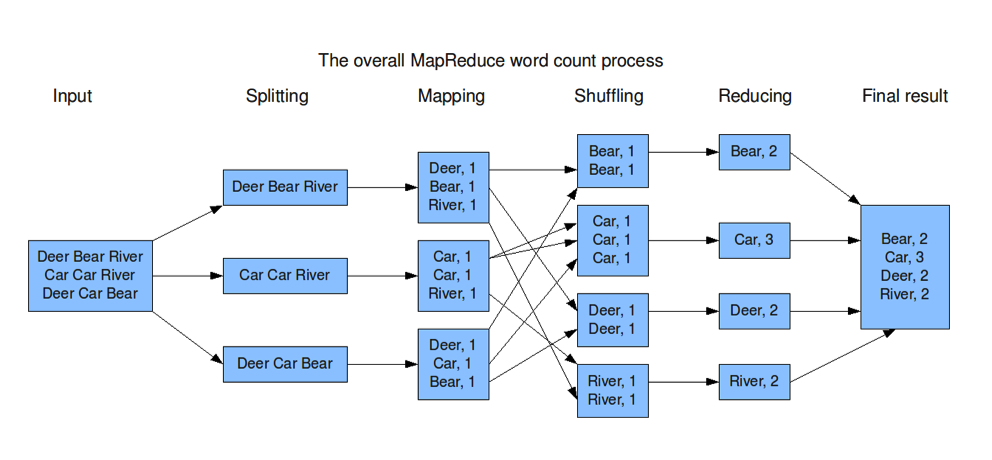
\includegraphics[width=1.0\textwidth]{bilder/2_6_1_wordcount.png}
\caption{Ein konkretes Word-Count-Beispiel für MapReduce  \protect\citeint{xi12}}
\label{fig:wordcount}
\end{figure}   
 


In Abbildung \ref{fig:wordcount} wird das MapReduce-Modell an einem praktischen Beispiel zur Wortzählung gezeigt. Bei MapReduce wird zunächst eine problemspezifische Map-Funktion definiert. Diese splittet die Ursprungsmenge in gleichgroße Teile, versieht unstrukturierte Worte in einem ersten Schritt mit Standardwerten, um so aus jedem unstrukturierten Datensatz ein Key-Value-Pair zu generieren. Im gezeigten Beispiel wird hier jedem Wert eine Eins als Anzahl zugeordnet. Im nächsten Schritt werden diese so gewonnenen Zwischen-Key-Value-Paare in einem Shuffling-Prozess klassifiziert und die so homogenisierten Pakete auf die Knoten im Cluster verteilt. Nun enthält jede Ausführungseinheit nur noch gleiche Wörter. Im Reduce-Schritt schließlich, werden die gleichartigen Wörter zu Gesamtmengen zusammengefasst, addiert und im Endergebnis aggregiert. 

An dem gezeigten Beispiel lässt sich gut erkennen, dass die einzelnen Ausführungsschritte jeweils parallelisiert und auf separate Knoten im Cluster verteilt werden können. Das Laufzeitsystem kümmert sich um die Details der Partitionierung der Eingabedaten, die Ressourcenverwaltung innerhalb des Clusters, das Behandeln von Fehlern und die Kommunikation zwischen den einzelnen Knoten. 
 

\section{Streaming Frameworks}
\label{section:streaming framworks}

Blablba

\section{Anwendungen von Graphen}
\label{section:anwendungen von graphen}

Blablba